\documentclass[a4paper, 12pt]{article}

\usepackage{hyperref}
\usepackage[warn]{mathtext}
\usepackage[utf8]{inputenc}
\usepackage[T2A]{fontenc}
\usepackage[english,russian]{babel}
\usepackage{multirow}
\usepackage{amsmath,amsfonts,amssymb,amsthm,mathtools}
\usepackage{indentfirst}
\DeclareSymbolFont{T2Aletters}{T2A}{cmr}{m}{it}
\usepackage{ gensymb }
\mathtoolsset{showonlyrefs=true}
\usepackage{euscript}
\usepackage{mathrsfs}
\usepackage[left=2cm,right=2cm,top=2cm,bottom=2cm]{geometry}
\usepackage{graphicx}
\usepackage{wrapfig}
\usepackage[rgb]{xcolor}
\hypersetup{
colorlinks=true,
urlcolor=blue
}


\title{Лабораторная работа}
\author{Гисич Арсений Б03-102}
\date{2022}

\begin{document}

	\begin{center}
		{\large МОСКОВСКИЙ ФИЗИКО-ТЕХНИЧЕСКИЙ ИНСТИТУТ (НАЦИОНАЛЬНЫЙ ИССЛЕДОВАТЕЛЬСКИЙ УНИВЕРСИТЕТ)}
	\end{center}
	\vspace{5 cm}
	{\Large
		\begin{center}
			{\bf Лабораторная работа 3.6.1}\\[0.2 cm]
			Спектральный анализ электрических сигналов
		\end{center}
	}
	\vspace{4 cm}
	\begin{flushright}
		{\Large Выполнил: \\
			\vspace{0.2 cm}
			Гисич Арсений \\
			\vspace{0.2 cm}
			Б03-102 \\}
	\end{flushright}
	\vspace{9 cm}
	\begin{center}
		Долгопрудный\\[0.1 cm]
		2022
	\end{center}
\thispagestyle{empty}

\section{Аннотация}

В работе изучается спектральный состав периодических электрических сигналов различной формы: последовательности прямоугольных импульсов, последовательности цугов и амплитудно модулированных гармонических колебаний. Спектры этих сигналов наблюдаются с помощью промышленного анализатора спектра и сравниваются с рассчитанными теоретически. 

\section{Теоретические сведения}

Представление периодического сигнала в виде суммы гармонических сигналов называется разложением в ряд Фурье.
	
Пусть заданная функция $f(t)$ периодически повторяется с частотой $\Omega_{1}=\dfrac{2\pi}{T},$ где $T$ --- период повторения. Ее разложение в ряд Фурье имеет вид
	
$$ f(t)=\dfrac{a_{0}}{2}+ \sum\limits_{n=1}^\infty [a_{n}\cos(n \Omega_{1}t)+b_{n}\sin(n \Omega_{1} t) ]$$
	
Здесь $\dfrac{a_{0}}{2}$ --- среднее значение функции $f(t)$,
	
$$ a_{n}=\dfrac{2}{T}\int\limits_{t_{1}}^{t_{1}+T}f(t)\cos(n \Omega_{1} t)dt, $$
	
$$ b_{n}=\dfrac{2}{T}\int\limits_{t_{1}}^{t_{1}+T}f(t)\sin(n \Omega_{1} t)dt. $$
	
Рассмотрим периодические функции, которые исследуются в нашей работе.
		
\textbf{Периодическая последовательность прямоугольных импульсов} (рис.~\ref{ris1}) с амплитудой $V_{0}$, длительностью $\tau$, частотой повторения $\Omega_{1}=\dfrac{2\pi}{T},$ где $T$ --- период повторения импульсов. Найдем коэффициенты разложения ряда Фурье:
	
$$\dfrac{a_{0}}{2}=V_{0}\dfrac{\tau}{T},$$
	
$$a_{n}=\dfrac{2}{T}\int\limits_{-\frac{\tau}{2}}^{\frac{\tau}{2}}V_{0}\cos(n \Omega_{1} t)dt=2V_{0}\dfrac{\tau}{T}\dfrac{\sin(n \Omega_{1} \frac{\tau}{2})}{n\Omega_{1}\frac{\tau}{2}} \sim \dfrac{\sin x}{x}.$$
	
Поскольку наша функция четная, все коэффициенты синусоидальных гармоник $b_{n}=0$. Спектр $a_{n}$ последовательности прямоугольных импульсов представлен на рис.~\ref{ris2} (изображен случай, когда $T$ кратно $\tau$).
		
		
\begin{figure}[h]
	\begin{minipage}[h]{0.5\linewidth}
		\center{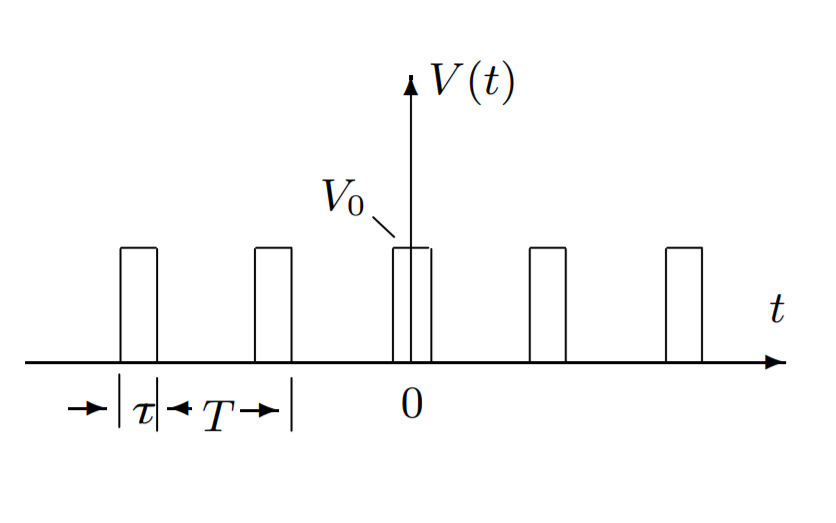
\includegraphics[width=0.9\linewidth]{sp1.png}}
		\caption{Прямоугольные импульсы}
		\label{ris1}
	\end{minipage}
	\begin{minipage}[h]{0.5\linewidth}
		\center{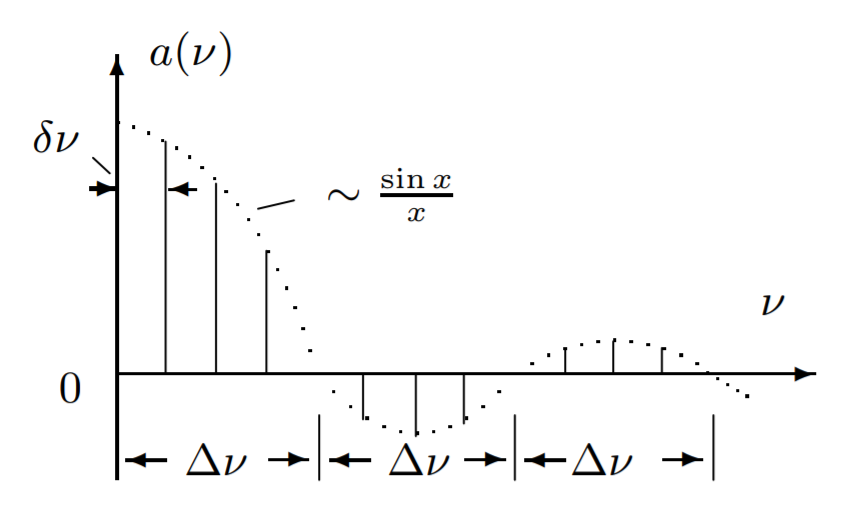
\includegraphics[width=0.9\linewidth]{sp2.png}}
		\caption{Спектр последовательности прямоугольных импульсов}
		\label{ris2}
	\end{minipage}
\end{figure}
	
Назовем \textit{шириной спектра} $\Delta \omega$ расстояние от главного максимума ($\omega =0$) до первого нуля огибающей, возникающего при $n=\dfrac{2\pi}{\tau \Omega_{1}}$. При этом 

$$\Delta \omega \tau \backsimeq 2 \pi $$

или 
	
\begin{equation}\label{neopr}
	\Delta \nu \Delta t \backsimeq 1
\end{equation}
		
Полученное соотношение взаимной связи интервалов $\Delta \nu$ и $\Delta t$ является частным случаем соотношения неопределенности в квантовой механике.
	
\textbf{Периодическая последовательность цугов} гармонического колебания $V_{0}\cos(\omega_{0}t)$ с длительностью цуга $\tau$ и периодом повторения $T$ (рис.~\ref{ris3}).
	
Функция $f(t)$ снова является четной относительно $t=0$. Коэффициент при $n$-й гармонике равен
	
$$a_{n}=\dfrac{2}{T}\int\limits_{-\frac{\tau}{2}}^{\frac{\tau}{2}}V_{0}\cos(\omega_{0}t)\cos(n \Omega_{1} t)dt=V_{0}\dfrac{\tau}{T} \bigg(\dfrac{\sin[(\omega_{0}-n\Omega_{1})\frac{\tau}{2}]}{(\omega_{0}-n\Omega_{1})\frac{\tau}{2}}+\dfrac{\sin[(\omega_{0}+n\Omega_{1})\frac{\tau}{2}]}{(\omega_{0}+n\Omega_{1})\frac{\tau}{2}} \bigg)$$ 
	
Зависимость для случая, когда $\frac{T}{\tau}$ равно целому числу, представлена на рис.~\ref{ris4}. Сравнивая спектр последовательности прямоугольных импульсов и цугов мы видим, что они аналогичны, но их максимумы сдвинуты по частоте на величину $\omega_{0}$.
	
\begin{figure}[h]
	\begin{minipage}[h]{0.5\linewidth}
		\center{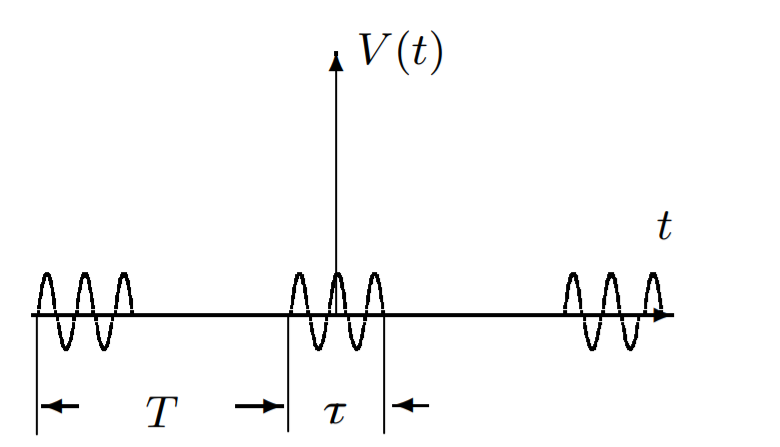
\includegraphics[width=0.9\linewidth]{sp3.png}}
		\caption{Последовательность цугов}
		\label{ris3}
	\end{minipage}
	\begin{minipage}[h]{0.5\linewidth}
		\center{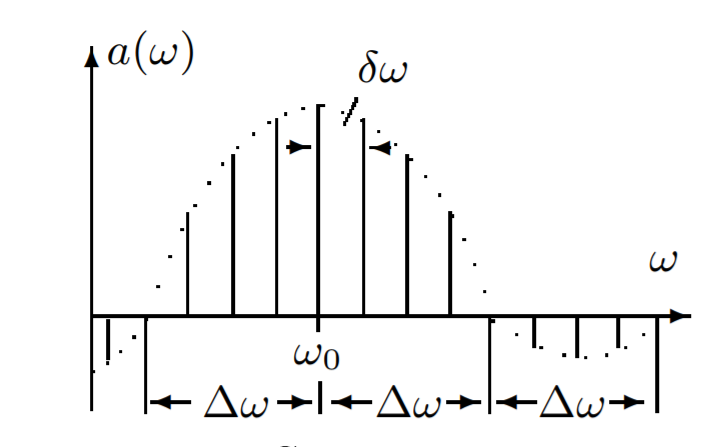
\includegraphics[width=0.9\linewidth]{sp4.png}}
		\caption{Спектр последовательности цугов}
		\label{ris4}
	\end{minipage}
\end{figure}

\textbf{Амплитудно-модулированные колебания.} Рассмотрим гармонические колебания высокой частоты $\omega_{0}$ , амплитуда которых медленно меняется по гармоническому закону с частотой $\Omega$ ($\Omega \ll \omega_{0}$) (рис.~\ref{ris5}):
	
$$f(t)=A_{0}[1+m\cos\Omega t]\cos \omega_{0}t.$$
	
Коэффициент $m$ называют \textbf{глубиной модуляции}. При $m<1$ амплитуда колебаний меняется от минимальной $A_{min}=A_{0}(1-m)$ до максимальной $A_{max}=A_{0}(1+m).$ Глубина модуляции может быть представлена в виде
	
\begin{equation}\label{m}
	 m=\dfrac{A_{max}-A_{min}}{A_{max}+A_{min}}
\end{equation}
	
Простым тригонометрическим преобразованием можно найти спектр амплитудно-модулированных колебаний:

\begin{equation}\label{a}
	f(t)=A_{0}\cos(\omega_{0} t)+\dfrac{A_{0}m}{2}\cos(\omega_{0}+\Omega)t+\dfrac{A_{0}m}{2}\cos(\omega_{0}-\Omega)t.
\end{equation}
		
\begin{figure}[h]
	\begin{minipage}[h]{0.5\linewidth}
		\center{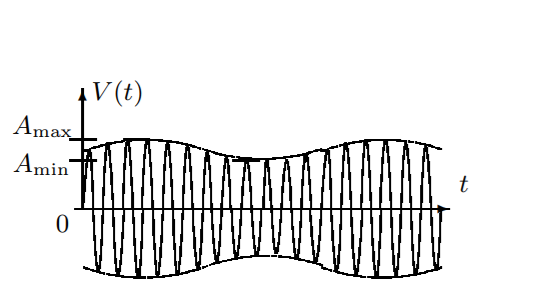
\includegraphics[width=0.9\linewidth]{sp5.png}}
		\caption{Модулированные гармонические колебания}
		\label{ris5}
	\end{minipage}
	\begin{minipage}[h]{0.5\linewidth}
		\center{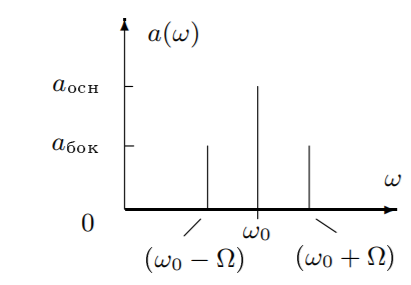
\includegraphics[width=0.9\linewidth]{sp6.png}}
		\caption{Спектр модулированных гармонических колебаний}
		\label{ris6}
	\end{minipage}
\end{figure}
		
Спектр таких колебаний содержит три составляющих: основную компоненту и две боковых (рис.~\ref{ris6}). Первое слагаемое в правой части представляет собой исходное немодулированное колебание с основной (несущей) частотой $\omega_{0}$ и амплитудой $a_{осн} = A_{0}$ . Второе и третье слагаемые соответствуют новым гармоническим колебаниям с частотами $\omega_{0} + \Omega$ и $\omega_{0} - \Omega$. Амплитуды этих двух колебаний одинаковы и составляют $\dfrac{m}{2}$ от амплитуды немодулированного колебания:
$a_{бок} = \dfrac{A_{0}m}{2}$. Начальные фазы всех трех колебаний одинаковы.

\section{Методика измерений}
	
\begin{enumerate}
		
\item \textbf{Экспериментальная установка А} для исследования спектра периодической последовательности прямоугольных импульсов представлена на рис.~\ref{A}. Сигнал с выхода генератора прямоугольных импульсов Г5-54 подается на вход анализатора спектра и одновременно  на вход Y осциллографа. С генератора импульсов на осциллограф подается также сигнал синхронизации, запускающий ждущую развертку осциллографа. При этом на экране осциллографа можно наблюдать саму последовательность прямоугольных импульсов, а на экране ЭЛТ анализатора спектра  распределение амплитуд спектральных составляющих этой последовательности.
					
\begin{figure}[h!]
	\centering
	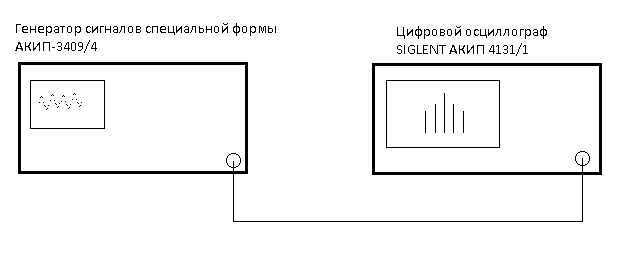
\includegraphics[width=\linewidth]{sp7.png}
	\caption{Cхема для исследования спектра периодической последовательности прямоугольных импульсов}
	\label{A}
\end{figure}
			
\item \textbf{Экспериментальная установка Б} для исследования спектра периодической последовательности цугов гармонических колебаний (рис.~\ref{B}) Генератор Г6-34 вырабатывает синусоидальные колебания высокой частоты. На вход АМ (амплитудная модуляция) генератора Г6-34 подаются прямоугольные импульсы с генератора Г5-54 и синусоида модулируется --- "нарезается" на отдельные куски --- цуги. Эти цуги с выхода генератора Г6-34 поступают на вход спектроанализатора и одновременно на вход Y осциллографа. Сигнал синхронизации подается на осциллограф с генератора импульсов.
		
\begin{figure}[h]
	\centering
	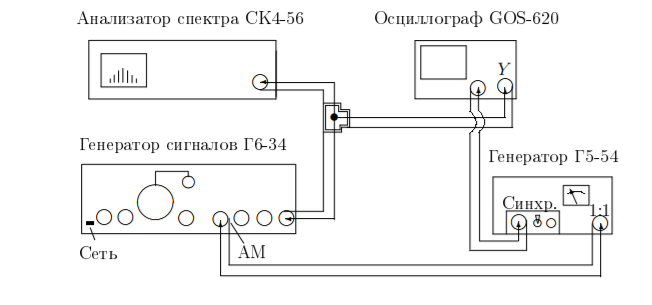
\includegraphics[width=0.8\linewidth]{sp8.png}
	\caption{Cхема для исследования спектра периодической последовательности цугов высокочастотных колебаний}
	\label{B}
\end{figure}
		
\item \textbf{Экспериментальная установка В} для исследования амплитудно-модулированного сигнала (рис.~\ref{C}). В генератор сигналов встроен модуляционный генератор, который расположен в левой части Г6-34. Синусоидальный сигнал с частотой модуляции $f_{мод}=1$ кГц подается с модуляционного генератора на вход АМ (амплитудная модуляция) генератора, вырабатывающего синусоидальный сигнал высокой частоты (частота несущей $\nu_{0}=25$ кГц). Амплитудно-модулированный сигнал с основного выхода генератора поступает на осциллограф и на анализатор спектра. 
		
\begin{figure}[h]
	\centering
	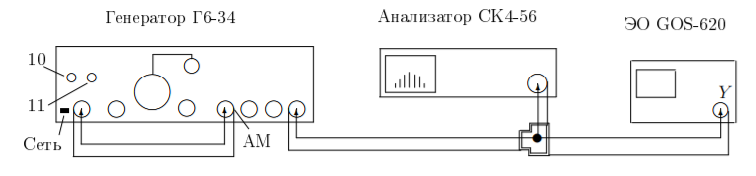
\includegraphics[width=0.8\linewidth]{sp9.png}
	\caption{Cхема для исследования спектра высокочастотного гармонического сигнала, промодулированного по амплитуде низкочастотным гармоническим сигналом}
	\label{C}
\end{figure}

\end{enumerate}

\section{Используемое оборудование}

\begin{enumerate}
    \item анализатор спектра;
    \item генератор прямоугольных импульсов и сигналов специальной формы;
    \item осциллограф;
\end{enumerate}

\section{Результаты измерений и обработка данных}

Параметры установки:
\begin{description}
\item{} $L = 26,5~см$
\item{} $SN = 3000~см^2$
\item{} $U_A = 1,230\pm0,025~кВ$
\end{description}

\begin{table}[h!]
\begin{center}
\begin{tabular}{|c|c|c|c|c|c|}
\hline
$I, A$ & $\sigma_{I}, A$ & $Ф, мВб$ & $\sigma_{Ф}, мВб$ & $B, мТл$ & $\sigma_{B}, мТл$ \\ \hline
0      & 0,005   & 0        & 0,05      & 0        & 0,2       \\ \hline
1,000  & 0,005   & 1,10     & 0,05      & 3,7      & 0,2       \\ \hline
1,500  & 0,005   & 1,60     & 0,05      & 5,3      & 0,2       \\ \hline
2,000  & 0,005   & 2,10     & 0,05      & 7,0      & 0,2       \\ \hline
2,500  & 0,005   & 2,60     & 0,05      & 8,7      & 0,2       \\ \hline
3,000  & 0,005   & 3,10     & 0,05      & 10,3     & 0,2       \\ \hline
3,500  & 0,005   & 3,80     & 0,05      & 12,7     & 0,2       \\ \hline
4,000  & 0,005   & 4,20     & 0,05      & 14,0     & 0,2       \\ \hline
4,500  & 0,005   & 4,50     & 0,05      & 15,0     & 0,2       \\ \hline
\end{tabular}
\end{center}
\caption{Результаты измерений калибровочной кривой при прямом направлении тока}
\label{tab1}
\end{table}

\section{Обсуждение результатов и выводы}

В данной работе был измерен удельный заряд электрона методами магнитной фокусировки и магнетрона. Результаты измерений:

$$\boxed{\begin{aligned}
&1,6\pm0,1\cdot 10^{11}~Кл/кг && \text{--- метод магнитной фокусировки} \\
&1,9\pm0,1\cdot 10^{11}~Кл/кг && \text{--- метод магнетрона} \\
\end{aligned}}$$

Полученные результаты согласуются в пределах погрешности с табличным значением~---~$1,76 \cdot 10^{11}~Кл/кг$. В методе магнитной фокусировки основной вклад в погрешность вносит погрешность определения коэффициента зависимости $B_ф(n)$. Вероятно, при более точной настройки фокусировки осциллографа можно более точно определить точки фокуса. В методе магнетрона основным источником погрешности является погрешность определения $B_{кр}$, так как низкая чувствительность амперметров не позволяет получить достаточно точек на кривой падения $I_A$ и хорошо промерить эту зависимость. При использовании более чувствительных измерительных приборов можно получить больше точек на этой кривой и, следовательно,точнее определить точки $B_{кр}$.

\end{document}